% Diagrama de conexión para la generación y medición de señal FM mediante entrada VCF
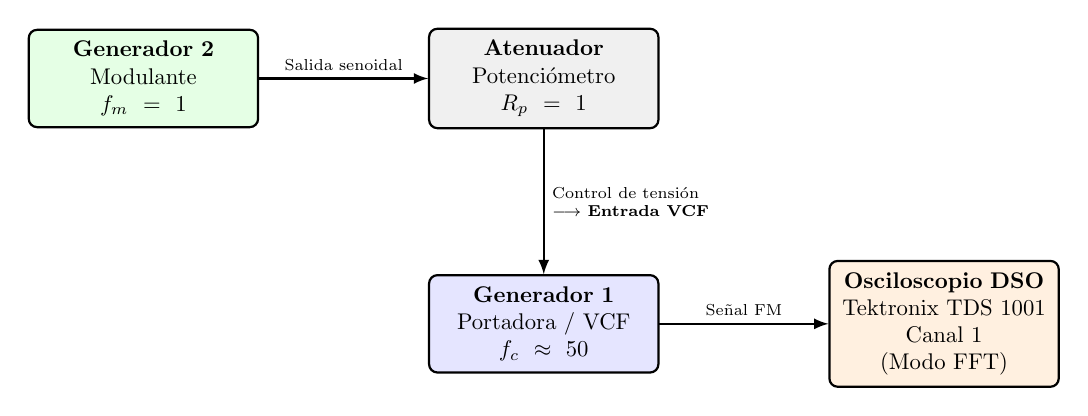
\begin{tikzpicture}[scale=0.82, transform shape,
    block/.style={rectangle, draw, fill=blue!8, rounded corners=3pt, thick, 
                  text width=3.2cm, text centered, minimum height=1.5cm, inner sep=5pt},
    line/.style={draw, -latex, thick}
]
    % Fila superior: Generador 2 (Modulante) y Potenciómetro Atenuador
    \node[block, fill=green!10] (g2) at (0, 2.2) {
        \textbf{Generador 2}\\Modulante\\$f_m = \qty{1}{\kilo\hertz}$
    };

    \node[block, fill=gray!12] (pot) at (6.2, 2.2) {
        \textbf{Atenuador}\\Potenciómetro\\$R_p = \qty{1}{\kilo\ohm}$
    };

    % Fila inferior: Generador 1 (Portadora y entrada VCF) y Osciloscopio Digital DSO
    \node[block, fill=blue!10] (g1) at (6.2, -1.6) {
        \textbf{Generador 1}\\Portadora / VCF\\$f_c \approx \qty{50}{\kilo\hertz}$
    };

    \node[block, fill=orange!12, text width=3.2cm] (osc) at (12.4, -1.6) {
        \textbf{Osciloscopio DSO}\\Tektronix TDS 1001\\Canal 1 (Modo FFT)
    };

    % Conexiones con etiquetas claras y sin superposiciones
    \path[line] (g2.east) -- node[above, font=\scriptsize] {Salida senoidal} (pot.west);
    \path[line] (pot.south) -- node[right, font=\scriptsize, align=left] {Control de tensión\\$\longrightarrow$ \textbf{Entrada VCF}} (g1.north);
    \path[line] (g1.east) -- node[above, font=\scriptsize] {Señal FM} (osc.west);
\end{tikzpicture}
